\documentclass{beamer}
\usetheme[pageofpages=of,% String used between the current page and the
                         % total page count.
          bullet=circle,% Use circles instead of squares for bullets.
          titleline=true,% Show a line below the frame title.
          alternativetitlepage=true,% Use the fancy title page.
       %   titlepagelogo=logo-polito,% Logo for the first page.
       %   watermark=watermark-polito,% Watermark used in every page.
       %   watermarkheight=100px,% Height of the watermark.
       %   watermarkheightmult=4,% The watermark image is 4 times bigger
                                % than watermarkheight.
          ]{Torino}

\setbeamertemplate{footline}{
  \begin{beamercolorbox}[wd=\paperwidth,ht=1ex,dp=1ex]{footline}
    \vspace{5pt} \hspace{1em} \insertframenumber/\inserttotalframenumber
  \end{beamercolorbox}
}

\author{Brendon J. Brewer}
\title{STATS 331 -- Introduction to Bayesian Statistics}
\institute{The University of Auckland}
\date{}


\linespread{1.3}
\usepackage{minted}
\usepackage[utf8]{inputenc}
\usepackage{dsfont}
\newcommand{\given}{\,|\,}


\begin{document}

\frame{\titlepage}

\begin{frame}
\centering
\Large
Bayesian T-Tests

\end{frame}


\begin{frame}
\frametitle{Plan}

\begin{itemize}
\item Today we will look at Bayesian equivalents of the famous $t$-test.\pause
\item We will have three different models, all with the same
sampling distribution. The differences will be in the priors.\pause
\item (i) an easy but unrealistic prior, (ii) a 2D
spike-and-slab prior in JAGS, and (iii) our first hierarchical prior.
\end{itemize}

\end{frame}

\begin{frame}
\frametitle{Fake Data from Ed Jaynes}

\begin{itemize}
\item Manufacturer A's widgets:
Mean lifetime = 42 hours, SD = 7.48 hours based on $N=9$.\pause
\item Manufacturer B's widgets:
Mean lifetime = 50 hours, SD = 6.48 hours based on $N=4$.\pause
\end{itemize}

Is one manufacturer better than the other?

\end{frame}

\begin{frame}
\frametitle{Boxplot}

\begin{center}
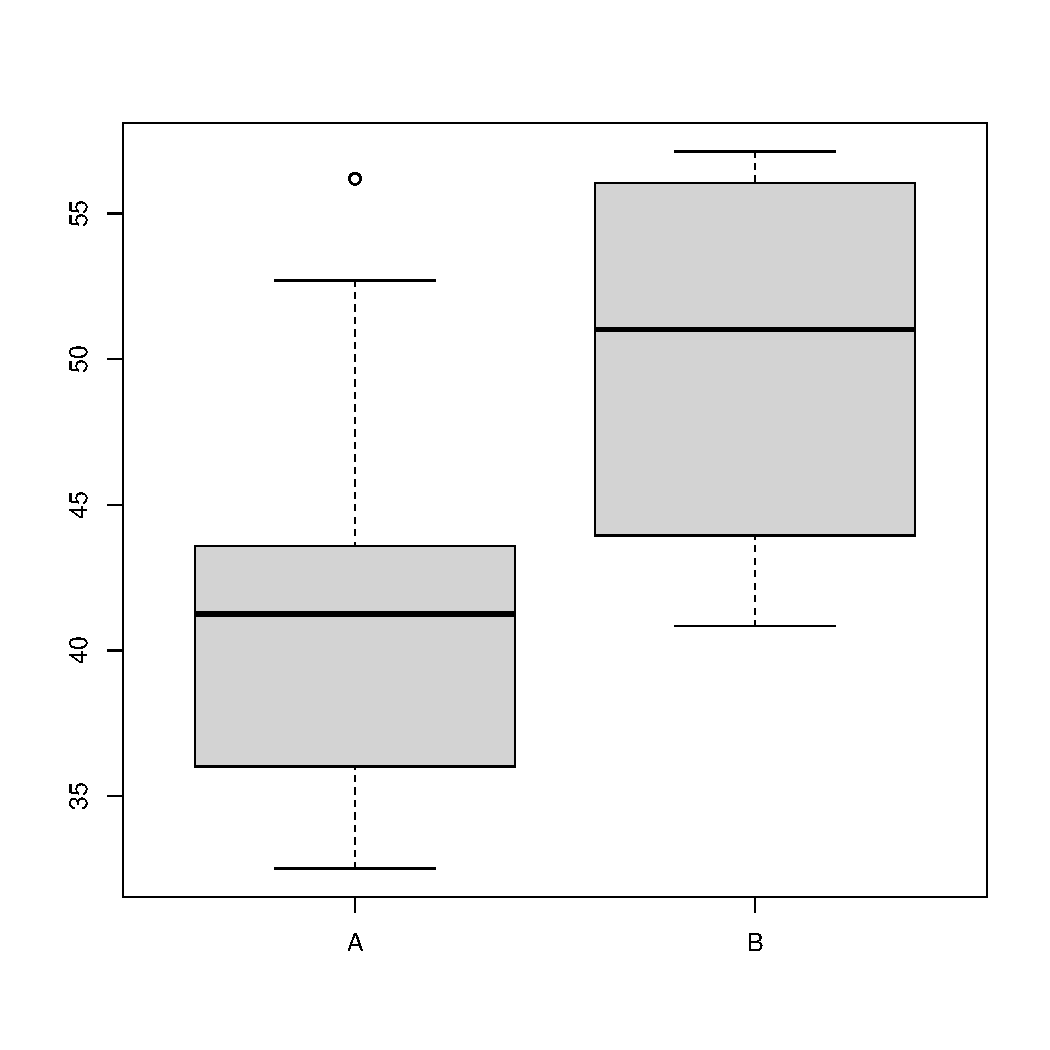
\includegraphics[width=0.6\textwidth]{images/widgets_boxplot.pdf}
\end{center}

\end{frame}


\begin{frame}
\frametitle{Classical $t$-test Hypotheses}

\begin{align}
H_0: \quad \mu_1 = \mu_2 \\
H_1: \quad \mu_1 \neq \mu_2
\end{align}
\end{frame}


\begin{frame}[fragile]
\frametitle{Classical $t$-test Results}
\footnotesize
\begin{minted}{r}
> t.test(data$x1, data$x2)

	Welch Two Sample t-test

data:  data$x1 and data$x2
t = -1.7461, df = 6.1694, p-value = 0.13
alternative hypothesis: true difference in means is not equal to 0
95 percent confidence interval:
 -19.136445   3.136445
sample estimates:
mean of x mean of y 
       42        50 
\end{minted}

\end{frame}


\begin{frame}[fragile]
\frametitle{Meaning of the $p$-value}
The p-value is the probability, assuming $H_0$ is true, that a dataset would
show this level of difference or greater.\\[0.5em]\pause

The posterior probability of $H_0$ is the probability that $H_0$ is true,
given the data. More what we want to know.
\end{frame}

\begin{frame}
\frametitle{Sampling Distribution Assumptions}
The classical $t$-test assumptions for the sampling distribution are the same
(apart from the interpretation of it) as what we will adopt:
\begin{align}
x_{1, i} \given \mu_1, \mu_2, \sigma &\sim \textnormal{Normal}(\mu_1, \sigma^2) \\
x_{2, i} \given \mu_1, \mu_2, \sigma &\sim \textnormal{Normal}(\mu_2, \sigma^2).
\end{align}
\pause

We will calculate joint posterior distributions for the
three  unknown parameters $\mu_1$, $\mu_2$, and
$\sigma$. From that, we can calculate the probability of $H_0$.


\end{frame}

\begin{frame}[fragile]
\frametitle{JAGS Code for Sampling Distribution}
The sampling distribution/likelihood code in JAGS is straightforward,
we just have to name the variables as they are named in the data:
\begin{minted}{r}
for(i in 1:N1)
{
    x1[i] ~ dnorm(mu1, 1/sigma^2)
}
for(i in 1:N2)
{
    x2[i] ~ dnorm(mu2, 1/sigma^2)
}
\end{minted}

\end{frame}


\begin{frame}[fragile]
\frametitle{Model 1: Priors}
In our first model, we will just set wide priors for the parameters.

\begin{minted}{r}
mu1 ~ dnorm(0, 1/1000^2)
mu2 ~ dnorm(0, 1/1000^2)
log_sigma ~ dunif(-10, 10)
sigma <- exp(log_sigma)
\end{minted}

\end{frame}


\begin{frame}[fragile]
\frametitle{Model 1: Results}
After running JAGS, we can get some posterior probabilities,
computed from the posterior samples.

\begin{minted}{r}
> mean(results$mu2 > results$mu1)
[1] 0.9437
> mean(results$mu2 == results$mu1)
[1] 0
\end{minted}
\pause

Why is the second result zero?



\end{frame}


\begin{frame}[fragile]
\frametitle{Model 1: Priors}
We got zero posterior probability for $H_0$ (that $\mu_1 = \mu_2$)
because we gave it zero prior probability! Take a look at the joint prior
for $\mu_1$ and $\mu_2$:
\vspace{-1.5em}
\begin{center}
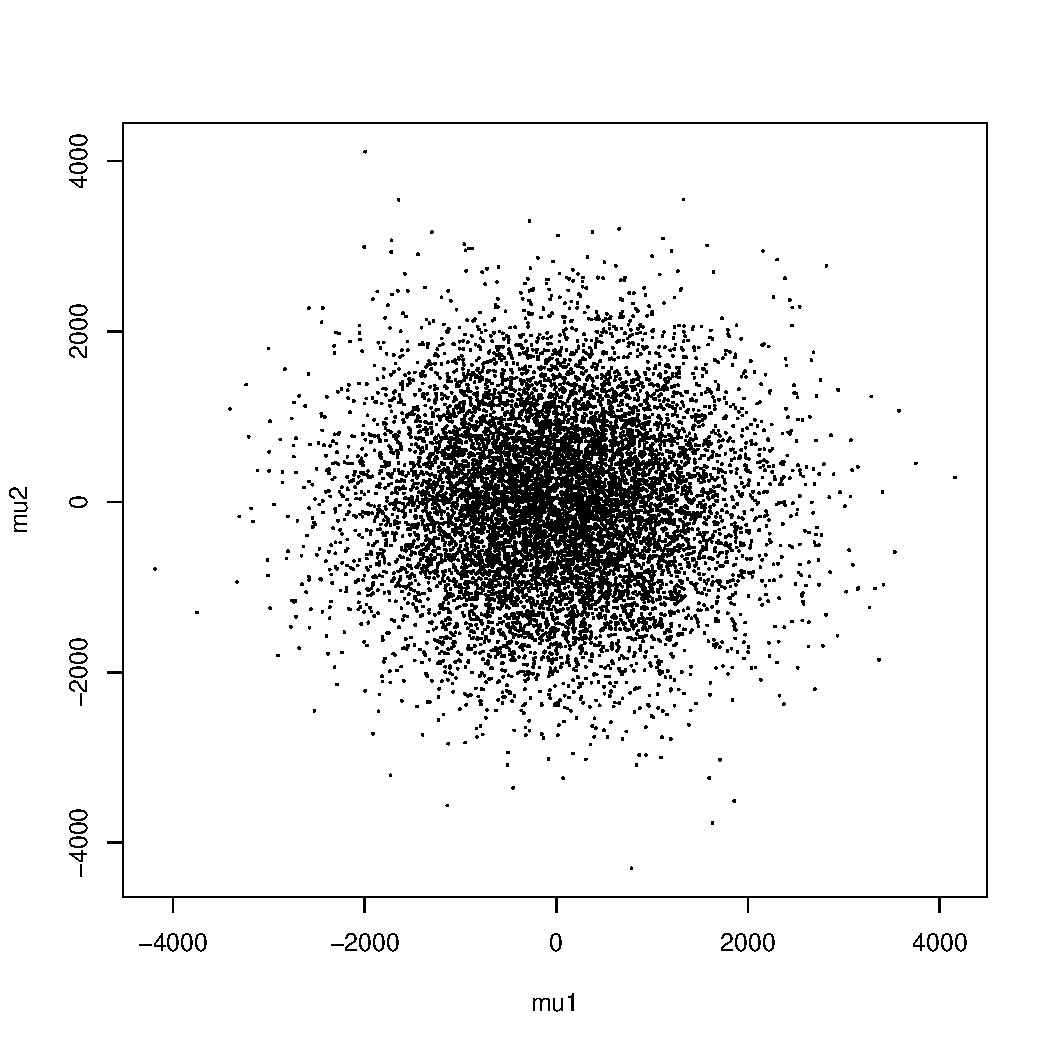
\includegraphics[width=0.5\textwidth]{images/ttest_prior1.pdf}
\end{center}


\end{frame}


\begin{frame}[fragile]
\frametitle{Model 1: Priors}
Not only does this prior assign zero probability to the hypothesis that the
two groups are equal, it assigns hardly any probability to the possibility
that they are even {\bf similar}.\\[0.5em]\pause

If we think $\mu_1$ and $\mu_2$ might be the same, we need some points
exactly on
the diagonal. If we think they might be different but similar, we need more
points {\em near} the diagonal.

\end{frame}

\end{document}

